% Author Vahid Partovi Nia
% Copyright Huawei Technologies
% Network Mind Team



\documentclass[12pt]{beamer}

\usetheme{Hannover}
\setbeamercolor{section in sidebar shaded}{fg=black}

\usecolortheme{beaver}
\beamertemplatenavigationsymbolsempty

%  \usebeamertemplate{navigation symbols}\hfill
%  \insertframenumber{}/\inserttotalframenumber}
  

\useoutertheme{sidebar}
\pgfdeclareimage[width=2.5\baselineskip]{institut-logo}{fig/mcgill_logo}
\setbeamertemplate{footline}
{\raisebox{-2ex}{\pgfuseimage{institut-logo}}
%  \hfill
\hspace{5cm}
  \usebeamertemplate{navigation symbols}
  \insertframenumber{}/\inserttotalframenumber
  \hspace{3.8cm}
YCBS255
}
%\setbeamertemplate{sidebar right}{}
  
\setbeamercolor{block title}{fg=darkred}
\setbeamercolor{local structure}{fg=darkred}

\setbeamercolor{palette sidebar secondary}{fg=darkgray, bg=white}



\usefonttheme{professionalfonts} % using non standard fonts for beamer


\makeatletter
\beamer@nav@subsectionstyle{hide/hide/hide}
\makeatother

\titlegraphic{\includegraphics[width=2cm]{fig/mcgill_logo}}




\usepackage{listings}
\usepackage{xcolor}
\def \y {\mathbf y}
\def \z {\mathbf z}
\def \Z {\mathbf Z}
\def \X {\mathbf X}
\def \A {\mathbf A}
\def \t {^\top}
\def \inv {^ {-1}}
\def \x {\mathbf x}
\def \bbeta {\boldsymbol \beta}
\def \eeps {\boldsymbol \varepsilon}
\def \TV {\mathrm{TV}}
\def \Radio {\mathrm{Radio}}
\def \Newspaper {\mathrm{Newspaper}}
\def \Sales {\mathrm{Sales}}
\def \Balance {\mathrm{Balance}}
\def \Default {\mathrm{Default}}
\def \M {\mathcal{M}}

\def \r {\mathbf{r}}
\def \e {\mathbf{e}}

\def \RSS {\mathrm{RSS}}

\def \E {\mathrm{E}}
\def \P {\mathbf{P}}

\def \V {\mathrm{V}}
\def \cor {\mathrm{cor}}

\def \SSigma {\boldsymbol{\Sigma}}
\def \LLambda {\boldsymbol{\Lambda}}
\def \pphi {\boldsymbol{\phi}}
\def \PPhi {\boldsymbol{\Phi}}
\def \mmu {\boldsymbol{\mu}}
\def \ttheta {\boldsymbol{\theta}}


\definecolor{capri}{rgb}{0.0, 0.75, 1.0}
\definecolor{darkcyan}{rgb}{0.0, 0.55, 0.55}
\definecolor{deepfuchsia}{rgb}{0.76, 0.33, 0.76}
\begin{document}
% no title and no author on sidebar
\title[]{Beyond Linearity}   
\author[]{Vahid Partovi Nia} 
\institute{Lecture 07}
\date{}


\makeatletter
  \begin{frame}[plain]
    \hspace*{-\beamer@leftsidebar}%
    \advance\textwidth by \beamer@leftsidebar\relax
    \beamer@leftsidebar=\z@
    \begin{minipage}{\textwidth}\par%
      \maketitle
    \end{minipage}
  \end{frame}
  \makeatother



\frame{\frametitle{Outline}\tableofcontents} 

\setbeamertemplate{sidebar left}[sidebar theme]

\section{Splines}
\frame{\frametitle{Splines}
Splines: another way of polynomial regression
}
\frame{\frametitle{univariate function approximation}
Suppose approximation of a good univariate function over a set of observed $(x_i, y_i), i=1,\ldots, n.$
$$y_i =f(x_i)+\varepsilon_i \approx \sum_{j} \beta_j b_j(x_i)$$
\begin{itemize}
\item polynomial base  $b_j(x_i) = x_i ^j$ 
\item Fourier base  
\item Wavelet base 
$$y_i \approx \sum_{j=1}^{2^k -1 } \beta^{(k)}_j b^{(k)}_j(x_i) $$
\end{itemize}
}


\frame{\frametitle{Piecewise polynomials}
\includegraphics[width=0.4\textwidth]{fig/fig5-1-01}
\includegraphics[width=0.4\textwidth]{fig/fig5-1-02}\\
\includegraphics[width=0.4\textwidth]{fig/fig5-1-03}
}

\frame{\frametitle{Cubic}
\includegraphics[width=0.4\textwidth]{fig/fig5-2-01}
\includegraphics[width=0.4\textwidth]{fig/fig5-2-02}\\
\includegraphics[width=0.4\textwidth]{fig/fig5-2-03}
\includegraphics[width=0.4\textwidth]{fig/fig5-2-04}
}


\frame{\frametitle{Splines}
B splines of order $m$ are piece-wise polynomial functions
\begin{eqnarray*}
h_0(x) &=& 1\\
h_1(x) &=& x \\
h_2(x) &=& x^2\\
h_{2+l}(x) &=& \{\max(0, x-\xi_l)\}^{3}
\end{eqnarray*}
}

\frame{\frametitle{Generalized ridge}
\begin{eqnarray*}
\hat \bbeta &=&   \min (\y - \mathbf K\bbeta )\t (\y - \mathbf K\bbeta ) + \lambda \bbeta\t \mathbf K \bbeta  \\
\end{eqnarray*}
Replace  $\min (\y - \mathbf K\bbeta )\t (\y - \mathbf K\bbeta )$ with $\max(0, 1-y_i \mathbf K\bbeta)$ to produce support vector machines.
}

\section{Nearest Neighbours}
\frame{\frametitle{}
$k$-Nearest Neighbours: Average surrounding points
}


\frame{\frametitle{}
\includegraphics[width=0.8\textwidth]{fig/smooth00}
}


\frame{\frametitle{}
\includegraphics[width=0.8\textwidth]{fig/smooth01}
}

\frame{\frametitle{}
\includegraphics[width=0.8\textwidth]{fig/smooth02}
}

\frame{\frametitle{}
\includegraphics[width=0.8\textwidth]{fig/smooth03}
}

\frame{\frametitle{}
\includegraphics[width=0.8\textwidth]{fig/smooth00}
}

\frame{\frametitle{}
\includegraphics[width=0.8\textwidth]{fig/smooth05}
}

\frame{\frametitle{}
\includegraphics[width=0.8\textwidth]{fig/smooth06}
}

\frame{\frametitle{}
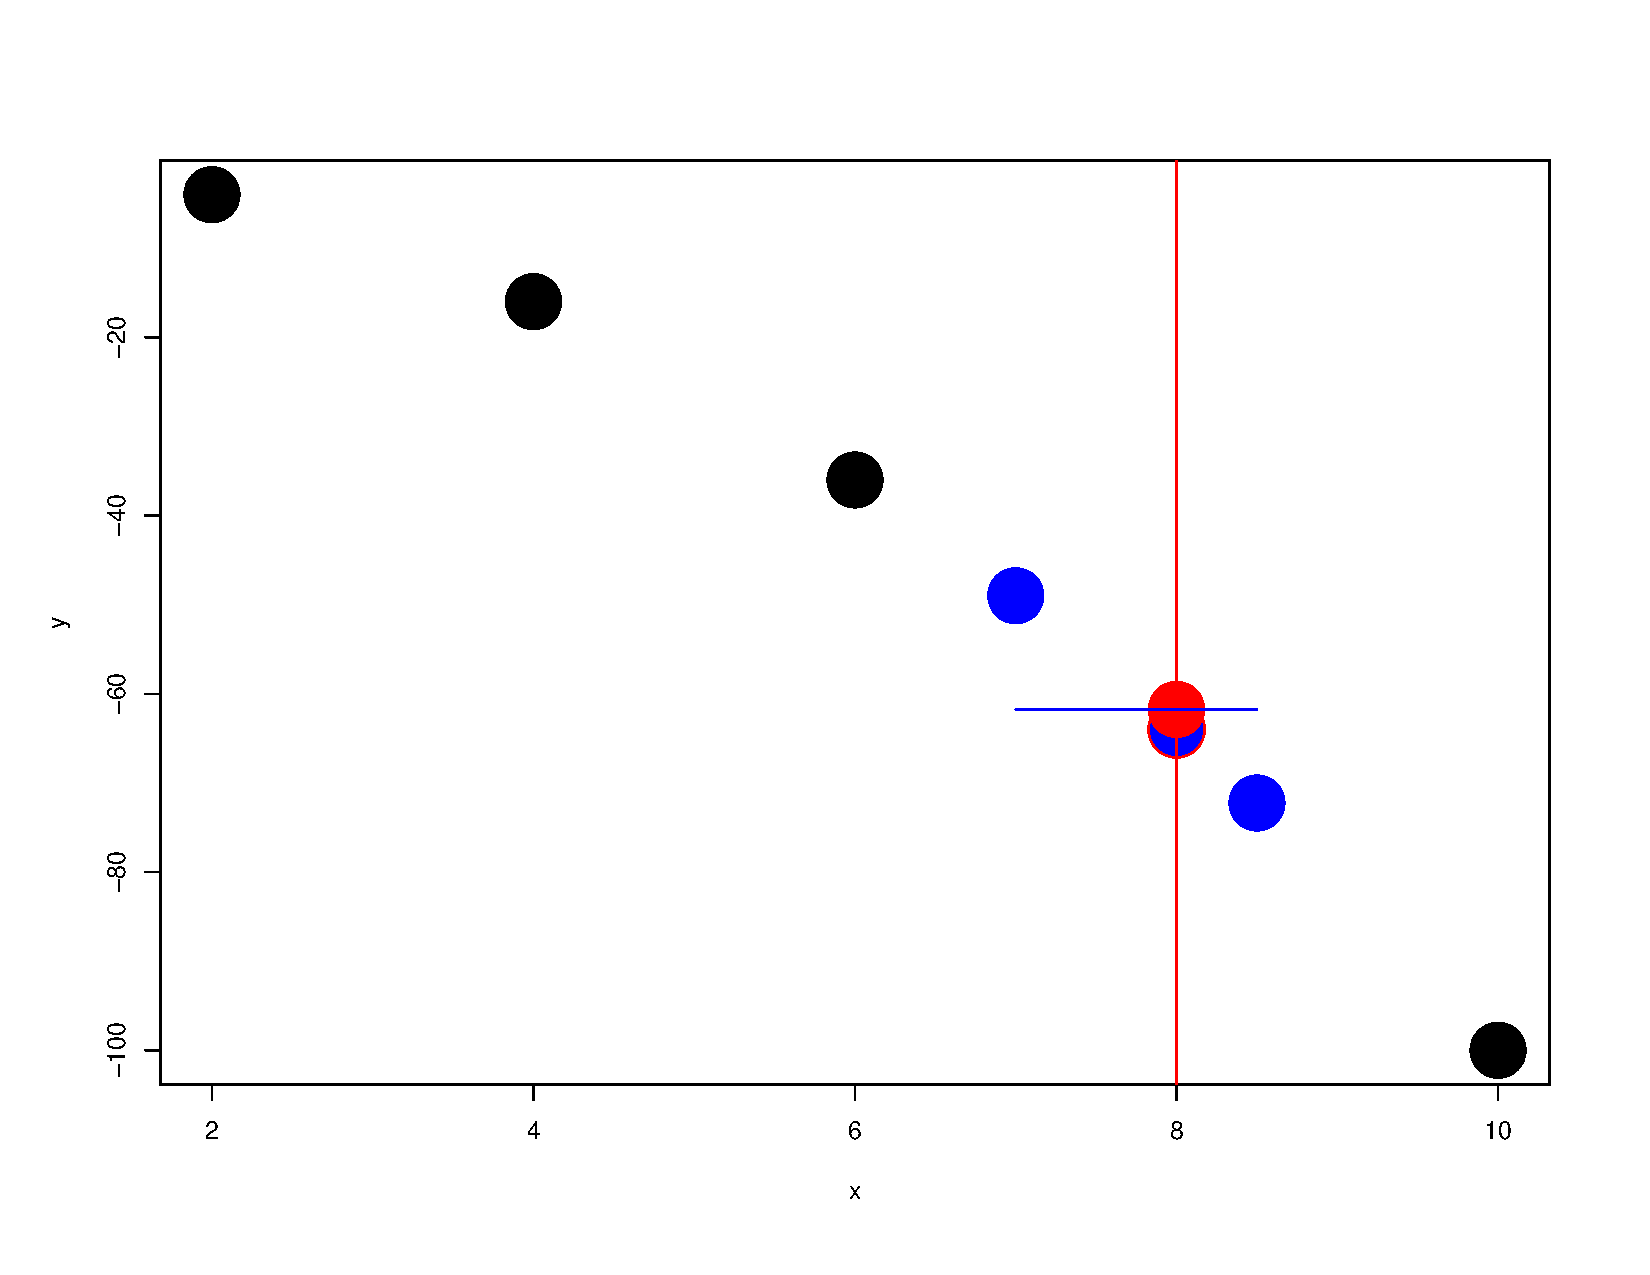
\includegraphics[width=0.8\textwidth]{fig/smooth07}
}
\section{Local Regression}
\frame{\frametitle{}
Local Regression: Average surrounding points smoothly
}



\frame{\frametitle{Smooth Kernel}
\includegraphics[width=0.5\textwidth]{fig/fig6-1-02}
}


\frame{\frametitle{Constant versus linear}
\includegraphics[width=0.3\textwidth]{fig/fig6-3-01} ~~
\includegraphics[width=0.3\textwidth]{fig/fig6-3-02}
}

\frame{\frametitle{transformed kernel}
\includegraphics[width=0.3\textwidth]{fig/fig6-4-01} ~~
\includegraphics[width=0.3\textwidth]{fig/fig6-4-02}
}

\frame{\frametitle{Kernel functions}
\includegraphics[width=0.8\textwidth]{fig/kernels}
}
\frame{\frametitle{Smooth histograms}
\includegraphics[width=0.8\textwidth]{fig/histsmooth}
}

\frame{\frametitle{}
Polynomial logistic regression using statsmodels
}

\begin{frame}[fragile]\frametitle{}
\tiny	
\begin{lstlisting}
import pandas as pd
path='data/'
filename = path+'Wage.csv'
wage = pd.read_csv(filename)
\end{lstlisting} 
\pause
\begin{lstlisting}
from sklearn.preprocessing import PolynomialFeatures
X1 = PolynomialFeatures(1).fit_transform(wage[['age']])
X2 = PolynomialFeatures(2).fit_transform(wage[['age']])
X3 = PolynomialFeatures(3).fit_transform(wage[['age']])
X4 = PolynomialFeatures(4).fit_transform(wage[['age']])
X5 = PolynomialFeatures(5).fit_transform(wage[['age']])
\end{lstlisting} 
\pause
\begin{lstlisting}
import statsmodels.api as sm
y = (wage['wage'] > 250).map({False:0, True:1})
lr = sm.GLM(y, X4, 
	family=sm.families.Binomial(sm.families.links.logit))
lr = lr.fit()
lr.summary()
\end{lstlisting} 
\end{frame}



\frame{\frametitle{Result}
\includegraphics[width=0.5\textwidth]{fig/logistic}
}

\begin{frame}[fragile]\frametitle{}
\tiny	
\begin{lstlisting}
age_grid = np.arange(20, 80).reshape(-1,1)
X_test = PolynomialFeatures(4).fit_transform(age_grid)
y_hat = lr.predict(X_test)

import matplotlib.pyplot as plt
%matplotlib inline
\end{lstlisting} 
\includegraphics[width=0.7\textwidth]{fig/logisticprob}
\end{frame}


\begin{frame}[fragile]\frametitle{}
\tiny	
\begin{lstlisting}
from statsmodels.nonparametric.smoothers_lowess import lowess

xy = lowess(wage['wage'], wage['age'], frac=0.1)
plt.scatter(wage['age'], wage['wage'], alpha=0.2)
plt.plot(xy[:,0],xy[:,1], 'red')
\end{lstlisting} 
\includegraphics[width=0.7\textwidth]{fig/lowess}
\end{frame}


%\begin{frame}[fragile]\frametitle{}
%\tiny	
%\begin{lstlisting}
%\end{lstlisting} 
%\end{frame}

%\begin{frame}[fragile]\frametitle{}
%\tiny	
%\begin{lstlisting}
%\end{lstlisting} 
%\end{frame}

%\begin{frame}[fragile]\frametitle{}
%\tiny	
%\begin{lstlisting}
%\end{lstlisting} 
%\end{frame}

%\begin{frame}[fragile]\frametitle{}
%\tiny	
%\begin{lstlisting}
%\end{lstlisting} 
%\end{frame}




%\frame{\frametitle{}
%\includegraphics[width=0.5\textwidth]{fig/}
%}

%\frame{\frametitle{}
%\includegraphics[width=0.5\textwidth]{fig/}
%}

%\frame{\frametitle{}
%\includegraphics[width=0.5\textwidth]{fig/}
%}
%

%\frame{\frametitle{}
%\includegraphics[width=0.5\textwidth]{fig/}
%}
%
%
%

\end{document}
